\Chapter{Ethernet}
\label{chap:ethernet}

\Paragraph{\acs{MAC} addresses}
\mode<article>{
A \ac{MAC} address is a unique identifier that is assigned to a \ac{NIC} for use as an address in communication within a network segment.
\ac{MAC} addresses are primarily assigned by device manufacturers and stored in read-only memory.
As such they are often referred to as the \emph{burned-in address}, or as a \emph{hardware address}, or \emph{physical address}.
Nowadays it is very often possible to change the \acs{MAC} adddress used on an interface.
}

\Paragraph{48 bits}
\mode<article>{
A \ac{MAC} address consists of 48~bits, most often displayed as six groups of two hexadecimal digits, separated by hyphens or colons (e.g.~02:\-00:\-33:\-aa:\-bb:\-cc).
Something the address is displayed as three groups of four hexadecimal digits, separated by dots, e.g. 0200.33aa.bbcc.%
   \footnote{It is important to note that hexadecimal numbers are not case-sensitive, meaning that the value of 4F is equivalent to that of 4f.}
}

\Paragraph{\acf{OUI}}
\mode<article>{
The first 24 bits of a \ac{MAC} address identify the vendor or manufacturer of the network card.
\Acp{OUI} are purchased from the \acs{IEEE} registration authority by the vendor.
They are used to make sure that -- in theory at least -- every \acs{MAC} address is unique.
}

\mode<article>{
\begin{extrainfo}
This is not the complete truth about \acs{MAC} addresses as there are two special bits in the \acs{OUI}.
The last two bits of the first byte have a special meaning.
The right-most bit indicates a multicast (or broadcast) address when set to one.
The left-most of those two special bits indicates a locally administered \acs{MAC} address when set to one.
The term `locally administered' means that the administrator of the machine has manually set the \acs{MAC} address to something -- and it is thus not guaranteed to be globally unique.
In this case, the first three bytes are not an \acl{OUI}.
See \cref{fig:mac-format} for the complete picture of a \acs{MAC} address.
\end{extrainfo}

\begin{figure}
\centering
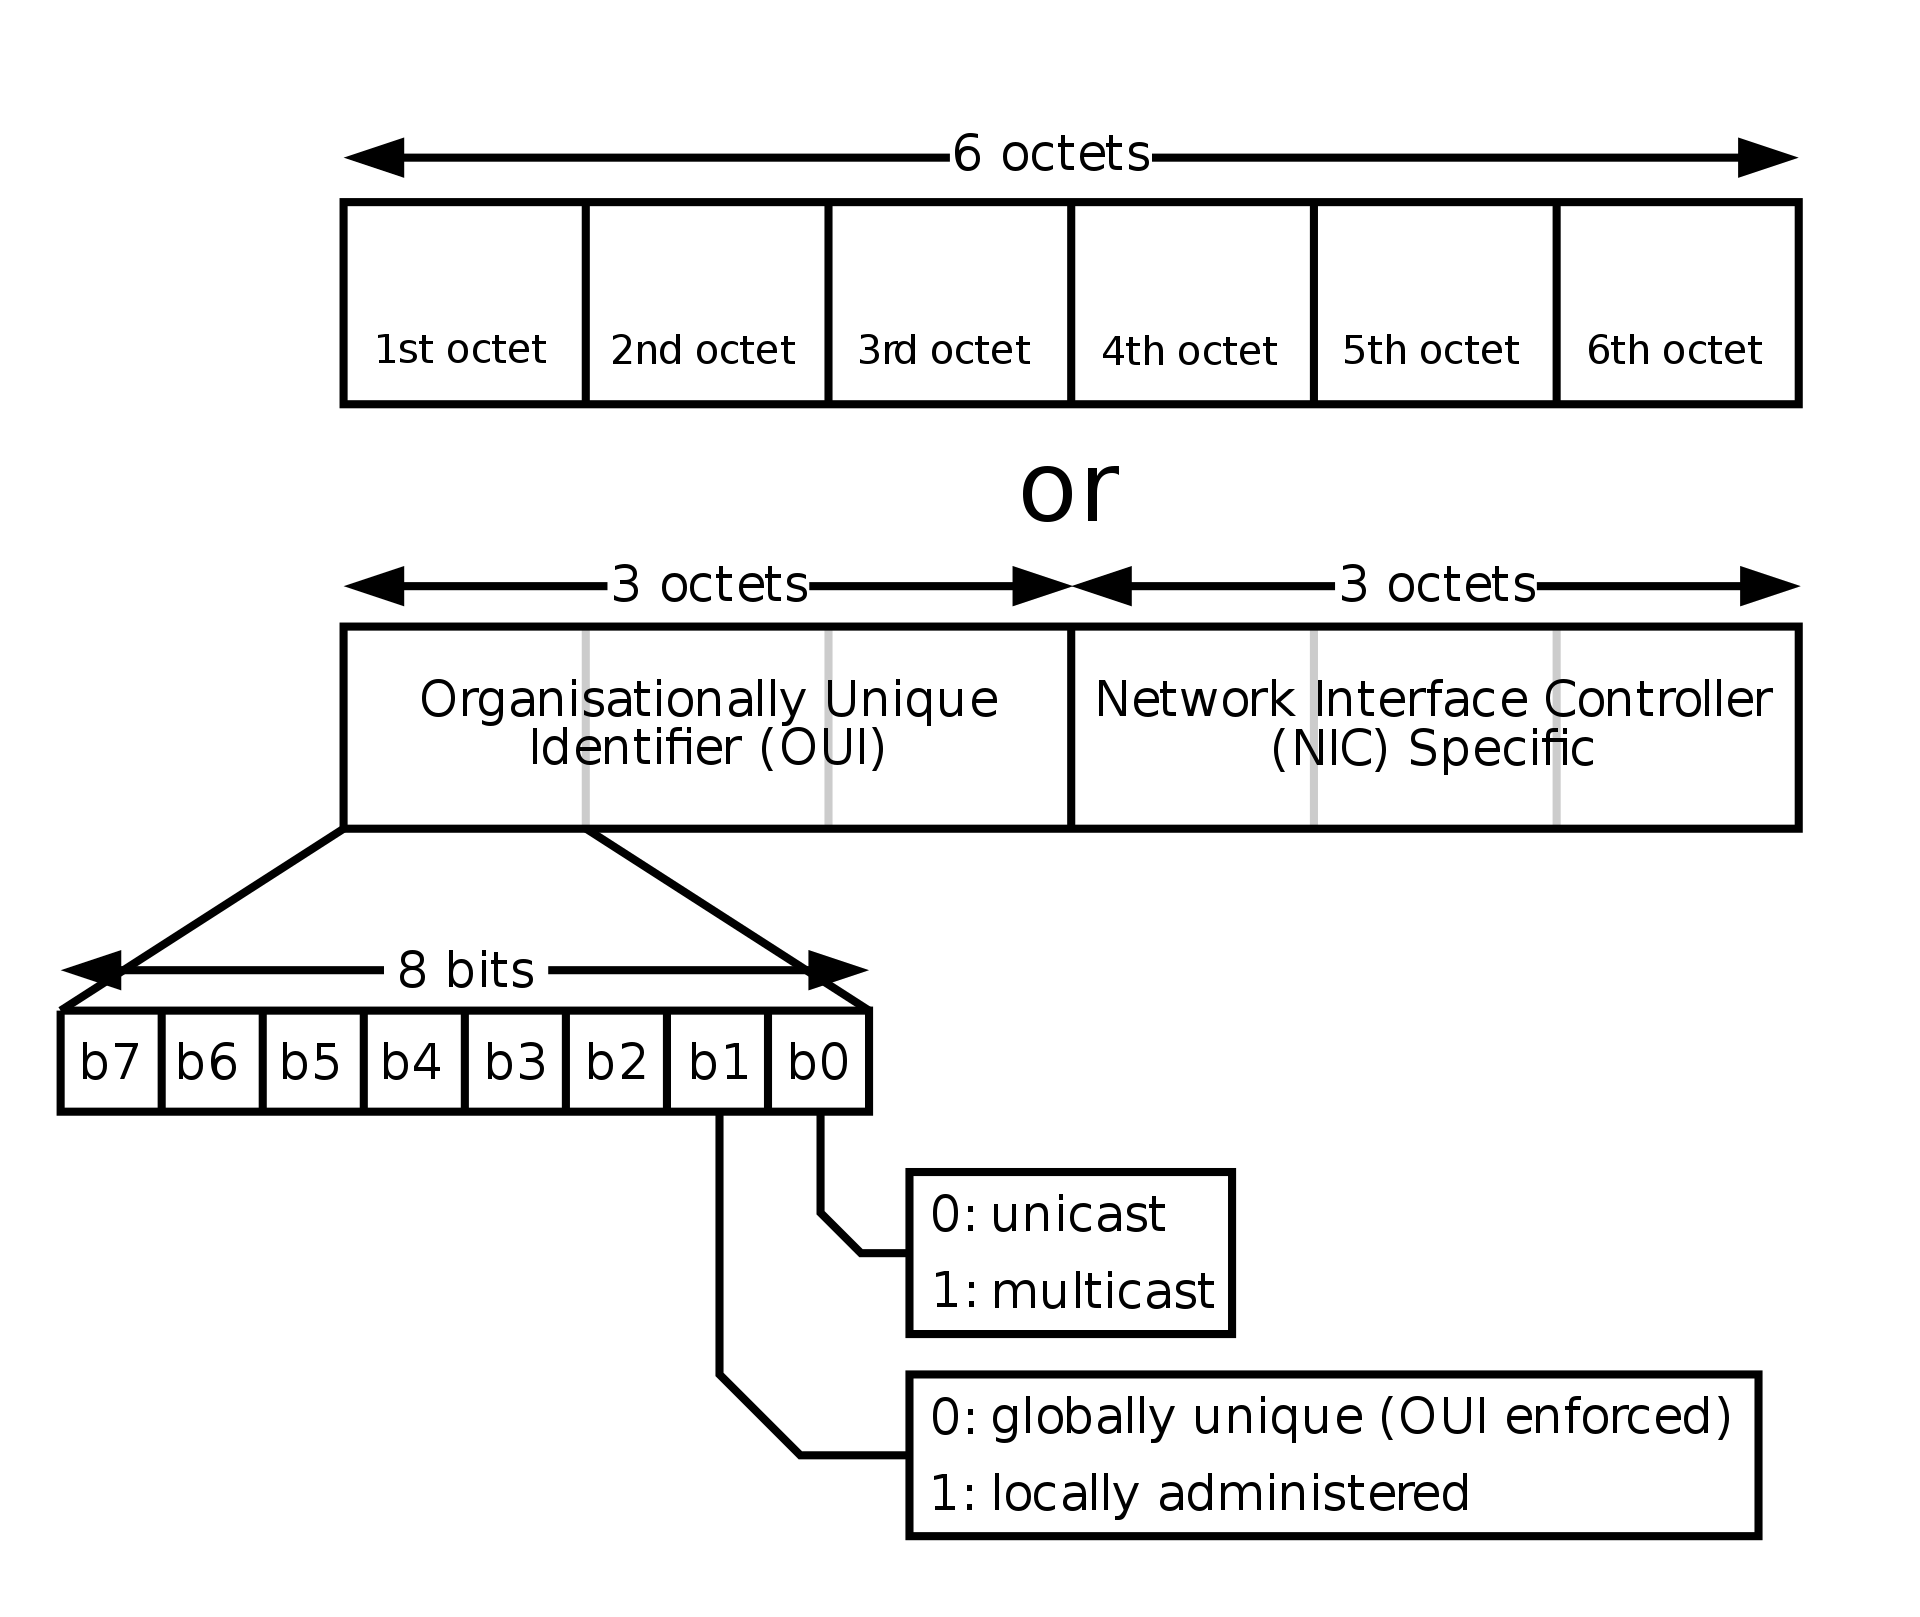
\includegraphics[width=.8\textwidth]{images/mac-address-format.png}
\caption{The \acs{MAC} address consists of two parts with the first part having two bits with special meaning}
\label{fig:mac-format}
\end{figure}
}

\Paragraph{1522 bytes}
\mode<article>{
Ethernet frames have a maximum size of 1522~bytes and a minimum frame size of 64~bytes.
Twenty-two bytes are used by the Ethernet header (18~bytes) and trailer (4~bytes) so that the encapsulated \acs{IP} packet has a maximum size of 1500~bytes.
}

\Paragraph{Ethernet header}

\Paragraph{Ethernet trailer}
\mode<article>{
The frame ends with a \acf{FCS}, which is a 32-bit \acf{CRC} used to detect any in-transit corruption of data.
}

\Paragraph{jumbo frames} 
\mode<article>{
Some implementations of Gigabit Ethernet and other higher-speed variants of Ethernet support larger frames, known as jumbo frames.
These frames can be up to 9022 bytes in size.
Jumbo frames are mainly used in data centres as the use of these larger frames require all intermediate devices to support them which is impossible to require from devices on the internet.
}


\Section{Ethernet switch}
\label{sec:ethernet-switch}

\Paragraph{hub}
\mode<article>{
An Ethernet hub has multiple \ac{IO} ports, in which a signal introduced at the input of any port appears at the output of every port except the original incoming.
A hub works at the physical layer (layer 1) of the \ac{OSI} model.
}

\Paragraph{\acs{MAC}-address table}
\mode<article>{
A network switch learns the identities of connected devices from incoming frames and then only forwards data to the port connected to the device to which it is addressed.
These learnt \acs{MAC} addresses are stored in the \ac{MAC}-address table.

The \acs{MAC}-address table contains the interface number that the frame came in on, the learnt \acs{MAC} address, the \acs{VLAN} that the frame belongs to, and a timer.
The timer serves to age out entries that are not used for a specific period of time.
By default, this timeout is three-hundred seconds on a Cisco switch.
}

\Paragraph{time to live?}
\mode<article>{
Ethernet has no \acl{TTL} field so when a loop gets created in the network, the frames will keep traversing the network, bringing the entire network down.
}

\Paragraph{\acf{STP}}
\mode<article>{
The \acl{STP} is a network protocol that builds a loop-free logical topology for Ethernet networks.
The basic function of \acs{STP} is to prevent bridge loops and the broadcast radiation that results from them.
\acs{STP} also allows a network design to include backup links providing fault tolerance if an active link fails.
}

\Paragraph{flavours of \acs{STP}}
\mode<article>{
In 2001, the \acs{IEEE} introduced \acf{RSTP} as 802.1w.
\acs{RSTP} provides significantly faster recovery in response to network changes or failures, introducing new convergence behaviors and bridge port roles to do this.
\acs{RSTP} was designed to be backwards-compatible with standard \acs{STP}.

\acs{STP} and \acs{RSTP} do not segregate switch ports by \acs{VLAN}.
However, in Ethernet switched environments where multiple \acsp{VLAN} exist, it is often desirable to create multiple spanning trees so that traffic on different \acsp{VLAN} uses different links.
Before the \acs{IEEE} published an \acs{STP} standard for \acsp{VLAN}, a number of vendors who sold \acs{VLAN}-capable switches developed their own \acs{STP} versions that were \acs{VLAN} capable.
Cisco developed, implemented and published the \acf{PVST} proprietary protocol and \acs{PVST+} which uses \abbr{802.1Q} \acs{VLAN} encapsulation.
Both standards implement a separate spanning tree for every VLAN.

The switch vendor Juniper Networks in turn developed and implemented its \acf{VSTP} to provide compatibility with Cisco's \acs{PVST}, so that the switches from both vendors can be included in one network.
Cisco also published a proprietary version of \acf{RSTP}.
It creates a spanning tree for each \acs{VLAN}, just like \acs{PVST}.
Cisco refers to this as \acf{RPVST}.

% TODO: add information on MST
}

\Paragraph{\acf{LAG}}
\mode<article>{
Link aggregation is the combining (aggregating) of multiple network connections in parallel by any of several methods, in order to increase throughput beyond what a single connection could sustain, to provide redundancy in case one of the links should fail, or both.
A \ac{LAG} is the combined collection of physical ports.
Other umbrella terms used to describe the concept include trunking%
   \footnote{Not to be confused with \acs{VLAN} trunking which is something entirely different that link aggregation trunking.}%
, bundling, bonding, channeling or teaming.
}

\Paragraph{managed switch}
\mode<article>{
Managed switches have one or more methods to modify the operation of the switch.
Common management methods include: a \ac{CLI} accessed via serial console, Telnet or \ac{SSH} (see \vref{chap:applications}), an embedded \ac{SNMP} agent allowing management from a remote console or management station, or a web interface for management from a web browser.
Examples of configuration changes that one can do from a managed switch include: enabling features such as \ac{STP} or port mirroring, setting port bandwidth, creating or modifying \acp{VLAN}, etc.

We will take a quick look at the following features of managed switches:
\begin{inlinelist}
\item \aclp{VLAN},
\item port security and \abbr{802.1X},
\item \acs{DHCP} snooping, and
\item \acl{DAI}.
\end{inlinelist}
}

\Paragraph{\acs{VLAN}}
\mode<article>{
   A \acf{VLAN} is any broadcast domain that is partitioned and isolated in a computer network at the data link layer.
   \acp{VLAN} work by applying tags to network frames and handling these tags in networking systems -- creating the appearance and functionality of network traffic that is physically on a single network but acts as if it is split between separate networks.
   In this way, \acp{VLAN} can keep network applications separate despite being connected to the same physical network, and without requiring multiple sets of cabling and networking devices to be deployed.
}

\Paragraph{access port}
\mode<article>{
An access port is an interface that is assigned to only one \acs{VLAN}.
Network frames sent and received on this port are not tagged with a \acs{VLAN}.
This type of interface is used towards end hosts such as printers, laptops, and workstations as they often do not understand \abbr{802.1Q} tags.
}


\Paragraph{trunk port}
\mode<article>{
A trunk port is an interface that is assigned to more than one \acs{VLAN}.
For the switch to be able to assign the network frame to the correct virtual network, all frames must be tagged with the correct \acs{VLAN} number.
}

\mode<article>{
\begin{extrainfo}
\paragraph{\abbr{802.1Q}}
\abbr{802.1Q} adds a 32-bit field between the source \acs{MAC} address and the ethertype field of the original frame.
Under \abbr{802.1Q}, the maximum frame size is extended from 1518~bytes to 1522~bytes.
The minimum frame size remains 64~bytes.
Two bytes are used for the \acf{TPID}, the other two bytes for \acf{TCI}.
The \acs{TCI} field is further divided into \acs{PCP}, \acs{DEI}, and \acs{VID}.

The \acl{TPID} is basically just the ethertype field.
It is a 16-bit field containing the hexadecimal value of 8100 which indicates an \acs{IEEE} \abbr{802.3Q}-tagged frame.
Receiving devices know that the next two bytes will contain \acs{VLAN} information and the two after that will contain the real ethertype value.

The \acs{PCP} and \acs{DEI} bits are used for quality of service and congestion control.
The \acl{VID} is a 12-bit field specifying the \acs{VLAN} to which the frame belongs.
The values of 0 and 4095 (f{}f{}f in hexadecimal) are reserved.
All other values may be used as \acs{VLAN} identifiers, allowing up to 4094~\acp{VLAN}.

\paragraph{native \acs{VLAN}}
Should a trunk port receive frames that lack an \abbr{802.3Q} tag, it is considered to belong to the \emph{native} \acs{VLAN} of that trunk port.
The network administrator can configure which \acs{VLAN} should be considered to be the native \acs{VLAN} for each interface.
\end{extrainfo}
}

\Paragraph{\acs{MAC} filtering}
\mode<article>{
   \ac{MAC} \emph{filtering} is a security access control method whereby the \acs{MAC} address assigned to each network card is used to determine access to the network.
   \ac{MAC} filtering on a network permits and denies network access to specific devices through the use of blacklists and whitelists.
   Many devices that support \acs{MAC} filtering do so on a device basis.
   Whitelisted \ac{MAC} addresses are allowed through any port on the device and blacklisted \acs{MAC} addresses are blocked on all ports.
   Other devices, such as Cisco Catalyst switches, support \acs{MAC} filtering on a port-by-port basis.
   Cisco refers to \acs{MAC} filtering as port security.
}

\Paragraph{\abbr{802.1X}}
\mode<article>{
\acs{IEEE} \abbr{802.1X} is an \acs{IEEE} standard for \ac{PNAC}.
It provides an authentication mechanism to devices wishing to attach to a \ac{LAN} or \ac{WAN}.

\abbr{802.1X} authentication involves three parties: a supplicant, an authenticator, and an authentication server.
The supplicant is a client device (such as a laptop) that wishes to attach to the \ac{LAN} or \ac{WAN}.
The authenticator is a network device that provides a data link between the client and the network and can allow or block network traffic between the two, such as an Ethernet switch or wireless access point.
The authentication server is typically a trusted server that can receive and respond to requests for network access, and can tell the authenticator whether the connection is to be allowed, and various settings that should apply to that client's connection.
Authentication servers typically run software supporting the \ac{RADIUS} protocol and \ac{EAP} framework.
}

\Paragraph{\acs{DHCP} snooping}
\mode<article>{
\ac{DHCP} snooping is a series of techniques applied to improve the security of a \ac{DHCP} infrastructure.
\ac{DHCP} snooping can be configured on \ac{LAN} switches to exclude rogue \ac{DHCP} servers and remove malicious or malformed \ac{DHCP} traffic.
In addition, information on hosts which have successfully completed a \ac{DHCP} transaction is accrued in a database of bindings which may then be used by other security or accounting features, such as \acl{DAI}.

The \ac{DHCP} snooping feature performs the following activities:
\begin{itemize}
\item it validates \acs{DHCP} messages received from untrusted sources and filters out invalid messages.
\item it rate-limits \acs{DHCP} traffic both from trusted and untrusted sources.
\item it builds and maintains the \acs{DHCP} snooping database, which contains information about untrusted hosts with leased \acs{IP} addresses.
\item it utilises the \acs{DHCP} snooping binding database to validate subsequent requests from untrusted hosts.
\end{itemize}
}

\Paragraph{\acl{DAI}}
\mode<article>{
\Acf{DAI} is a security feature that validates \acs{ARP} packets in a network.
\Acl{DAI} allows a network administrator to intercept, log, and discard \ac{ARP} packets with invalid \acs{MAC}-address-to-\acs{IP}-address bindings.
This capability protects the network from certain man-in-the-middle attacks.
}
\slide{\acf{DAI}}

\Paragraph{layer-3 switch}
\mode<article>{
As engineers continue to advance in their field, they have developed the ability to create larger and more complex chips.
This advancement allows for the integration of more complex logic into network switches.
Layer-3 switches, in particular, have the capability to route packets in hardware based on \acs{IP} addresses, effectively functioning as routers.
As a result, it has become increasingly convenient to implement a layer-3 switch into network infrastructure, as it combines the functionality of both routers and traditional switches.
}